
% ===========================
\chapter{Konzept}
\label{konzept}
% ===========================

Wie in Abschnitt \ref{grundlagen_fahren} beschrieben, stellt die Sicherung von hochautomatisierten \ac{FAS} die Automobilindustrie vor große Herausforderungen. Die Menge der bekannten Fahrszenarien ist nur eine Teilmenge aller Szenarien, die zukünftige \ac{FAS} abdecken müssen. Diese Beziehung ist schematisch in Abbildung \ref{fig_teilmenge_fahrszenarien} dargestellt. Die Folge ist eine steigende Anzahl benötigter Testkilometer, die in Zukunft mit ökonomischem Aufwand nicht mehr umsetzbar sein wird. Es müssen neue Methoden gefunden werden, relevante Szenarien für die Generierung von Testfällen zu identifizieren, um die Sicherung von hochautomatisierten \ac{FAS} mit ökonomischen Aufwand garantieren zu können.

Genau hier soll diese Arbeit einen Beitrag leisten. Das Ziel, wie bereits in Abschnitt \ref{einleitung_zielsetzung} erläutert, ist die Identifikation von bisher unbekannten Fahrszenarien. Die Grundidee ist es einen Klassifikator mit einem großen Anteil synthetischer Daten und einem kleinen Anteil realer Daten von bisher bekannten Szenarien zu trainieren. Dieser Klassifikator kann dann bekannte Szenarien erkennen, liefert aber keine eindeutigen Ergebnisse bei bisher unbekannten Szenarien. Mit dieser Methodik soll es möglich sein bisher unbekannte Fahrszenarien zu identifizieren, um auf der Basis neue Testfälle für die Sicherung hochautomatisierter Fahrfunktionen zu generieren.

\begin{figure}[h]
\centering
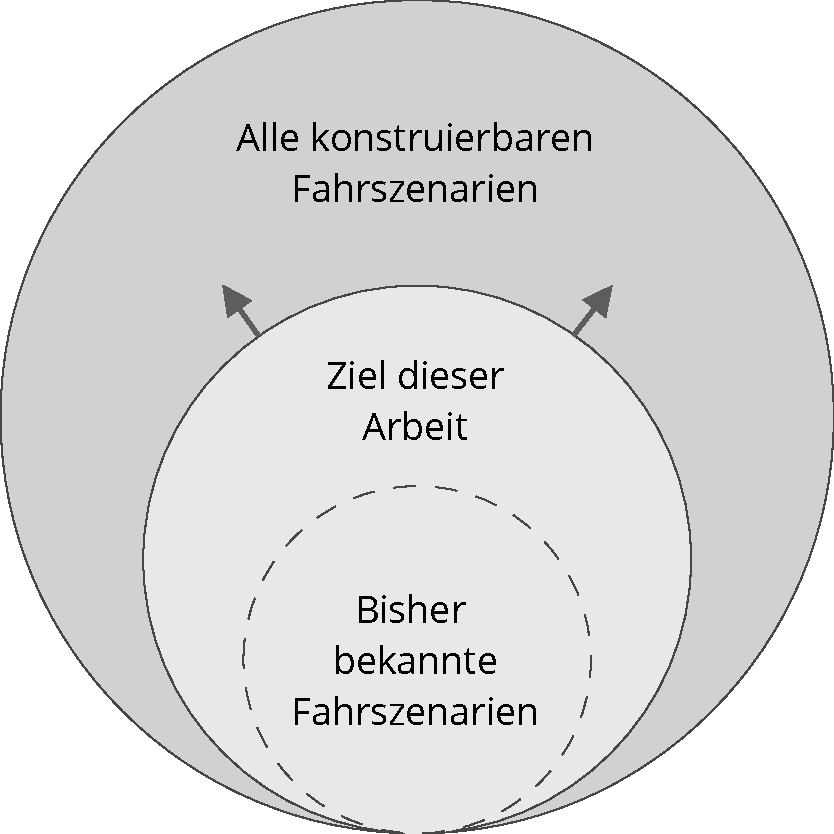
\includegraphics[scale=0.5]{teilmenge_fahrszenarien.pdf}
\caption{Beziehung zwischen bekannten und unbekannten Fahrszenarien}
\label{fig_teilmenge_fahrszenarien}
\end{figure}

In dieser Arbeit soll ein Proof-of-Concept für diese Methodik entwickelt werden. Dafür wird im folgenden Abschnitt \ref{konzept_struktur} das Konzept im Detail und die Vorgehensweise vorgestellt. Anschließend wird in Abschnitt \ref{konzept_methodik} die Methodik erklärt mit welcher dieses Konzept umgesetzt werden soll.


% ===========================
\section{Struktur}
\label{konzept_struktur}
% ===========================

Im ersten Schritt der Umsetzung werden bestimmte Fahrszenarien ausgewählt und wie in Abschnitt \ref{grundlagen_fahren_szenarien} definiert. In dieser Arbeit werden Szenarien auf der Ebene der \textit{logischen Szenarien} definiert. Nachdem Szenarien ausgewählt und definiert sind, werden synthetische und reale Daten für das Training eines Klassifikators benötigt.

Für die Generierung von synthetischen Daten wird mit der Simulationssoftware CarMaker gearbeitet. Mit dieser Software können das Ego-Fahrzeug, Straßen, Verkehr und die Trajektorien aller Fahrzeuge generiert und beliebig verändert werden. Die Idee ist es, Fahrten des Ego-Fahrzeugs zu simulieren, entsprechende Bild- und Signaldaten aufzuzeichnen und die Bilddaten anhand der Signaldaten zu labeln. Auf diese Weise können ohne großen Aufwand beliebig viele synthetische Daten erzeugt und gelabelt werden. Mit CarMaker können sowohl Rohdaten, wie zum Beispiel Radarsignale des Ego-Fahrzeugs, als auch abstrakte Informationen, wie die Position und Geschwindigkeit von anderen Objekten, simuliert werden. Amersbach und Winner \cite{amersbach2017functional} stellen einen Ansatz für die funktionale Dekomposition von hochautomatisierten \ac{FAS} vor. In diesem Ansatz werden Informationen über sechs Schritte, von den Ground Truth Daten über die Szenenerkennung bis zur entsprechenden Aktion des Ego-Fahrzeugs, abgeleitet. Ein Schema dieses Ansatzes ist in Abbildung \ref{fig_functional_decomposition} dargestellt. In dieser Arbeit werden Signaldaten generiert, die nach Schicht 1 (e.g. Geschwindigkeit des Ego-Fahrzeugs) und Schicht 2 (e.g Position des vorausfahrenden Fahrzeugs) eingeordnet werden können. Für das Labeling der Bilddaten werden die Signaldaten definiert die für das Labeling benötigt werden und dann mit CarMaker zusammen mit den Bilddaten generiert. Jeder generierte Zeitpunkt stellt eine Szene, wie in Abschnitt \ref{grundlagen_fahren_szenarien} beschrieben, dar und wird mit den entsprechenden Signaldaten nach festgelegten Regeln klassifiziert und gelabelt. Die Aneinanderreihung von mehreren Szenen ergibt schließlich ein Szenario.

\begin{figure}[h]
\centering
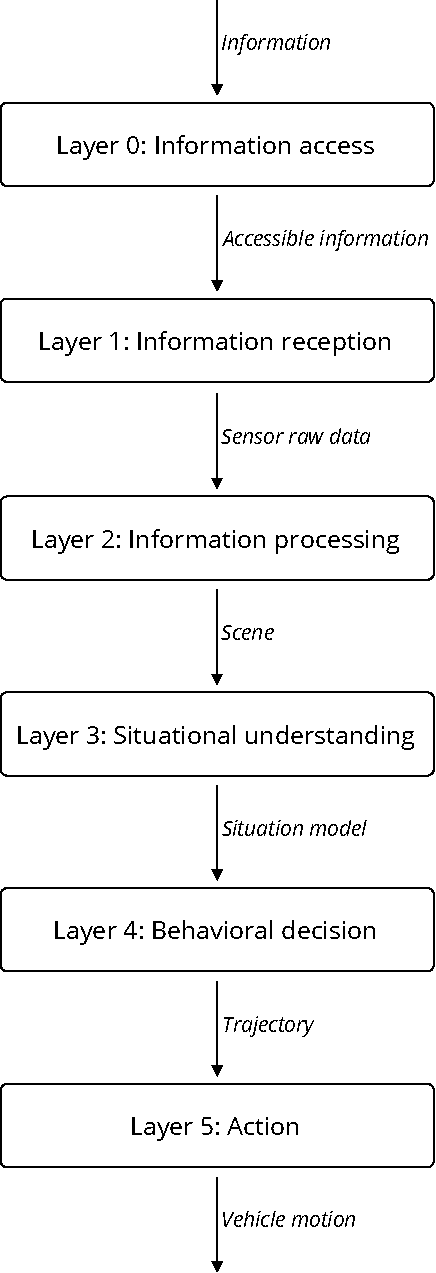
\includegraphics[scale=0.5]{functional_decomposition.pdf}
\caption{Schema der funktionalen Dekomposition \cite{amersbach2017functional}}
\label{fig_functional_decomposition}
\end{figure}

 Bei der Simulation können eine Vielzahl an 





- Definition von Fahrszenarien
- Simulation von Fahrten mit diesen Szenarien
- funktionale Dekomposition
- Extraktion und Labeling der Fahrszenarien
- Extraktion von Reale Fahrszenarien
- Training NN mit synthetischen und realen
- Evaluation mit realen Fahrszenarien



Für die Generierung von synthetischen Daten 



Gleichzeitig bleibt der Aufwand für das Labeling der Daten überschaubar, weil die synthetischen Daten automatisiert gelabelt werden können und die realen Daten nur einen geringen Anteil ausmachen sollen.

% ===========================
\section{Methodik}
\label{konzept_methodik}
% ===========================

Lorem ipsum dolor sit amet, consetetur sadipscing elitr, sed diam nonumy eirmod tempor invidunt ut labore et dolore magna aliquyam erat, sed diam voluptua. At vero eos et accusam et justo duo dolores et ea rebum. Stet clita kasd gubergren, no sea takimata sanctus est Lorem ipsum dolor sit amet.  






